\documentclass[tikz,border=9pt]{standalone}
\usepackage{amsmath,amssymb}
\usetikzlibrary{arrows.meta,positioning,calc}
\begin{document}
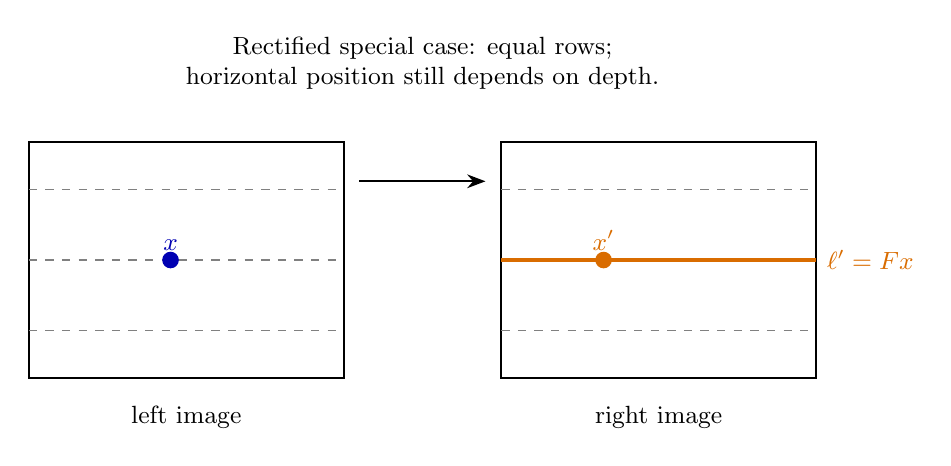
\begin{tikzpicture}[font=\small,arr/.style={-{Stealth},thick},box/.style={draw=blue!55!black,rounded corners,fill=blue!4,align=center,text width=2.9cm,minimum height=1.05cm}]

\foreach \offset/\name in {0/left,6/right}{
\draw[thick] (\offset,0) rectangle (\offset+4,3);
\foreach \y in {.6,1.5,2.4}{\draw[gray,dashed] (\offset,\y)--(\offset+4,\y);}
\node at (\offset+2,-.5){\name\ image};}
\fill[blue!70!black] (1.8,1.5) circle(3pt) node[above]{$x$};
\draw[very thick,orange!85!black] (6,1.5)--(10,1.5) node[right]{$\ell'=Fx$};
\fill[orange!85!black] (7.3,1.5) circle(3pt) node[above]{$x'$};
\draw[arr] (4.2,2.5)--(5.8,2.5);
\node[align=center] at (5,4){Rectified special case: equal rows;\\horizontal position still depends on depth.};

\end{tikzpicture}
\end{document}
